%
% File acl2018.tex
%
%% Based on the style files for ACL-2017, with some changes, which were, in turn,
%% Based on the style files for ACL-2015, with some improvements
%%  taken from the NAACL-2016 style
%% Based on the style files for ACL-2014, which were, in turn,
%% based on ACL-2013, ACL-2012, ACL-2011, ACL-2010, ACL-IJCNLP-2009,
%% EACL-2009, IJCNLP-2008...
%% Based on the style files for EACL 2006 by 
%%e.agirre@ehu.es or Sergi.Balari@uab.es
%% and that of ACL 08 by Joakim Nivre and Noah Smith

\documentclass[11pt,a4paper]{article}
\usepackage[hyperref]{vocabbysty}

\usepackage{times}
\usepackage{latexsym}
\usepackage{graphicx}
\usepackage{subfig}
\usepackage[most]{tcolorbox}
\usepackage{lipsum}

\graphicspath{ {./images/} }
\aclfinalcopy % Uncomment this line for the final submission
\def\aclpaperid{***} %  Enter the acl Paper ID here

%\setlength\titlebox{5cm}
% You can expand the titlebox if you need extra space
% to show all the authors. Please do not make the titlebox
% smaller than 5cm (the original size); we will check this
% in the camera-ready version and ask you to change it back.

\newcommand\BibTeX{B{\sc ib}\TeX}

\title{Structured vocabulary learning with in the context of learner domain}

\author{Haemanth Santhi Ponnusamy \qquad Himanshu Bansal \\\\
  International Studies of Computational Linguistics(ISCL) \\
  Eberhard Karls Universität Tübingen\\
  Germany \\\\ \tt \small \{haemanth.santhi-ponnusamy,himanshu.bansal\}@student.uni-tuebingen.de}

\date{}

\begin{document}
\maketitle
\begin{abstract}
  We propose a vocabulary learning approach targeted on the set of learners
  who already posses some basic skills in a language and bored of the
  traditional method of learning new words. Our design 
  structures the vocabulary space to estimate the learner's
  level in lesser number of interactions and track their performance efficiently.
  It also provides a great advantage in auto-generating the content
  for the entire learning process with almost zero human effort. We allow the
  learner to choose the text of their own interest. Then all the activities and
  feedback are generated only from the chosen text.
\end{abstract}

\section{Introduction}
Vocabulary learning is an open ended task as the languages are vast and still
evolving with the addition of new words now and then. This makes it hard for the vocabulary learners to sense the progress. Popular vocabulary learning applications such as Duolingo, Memrise, LingoDeer, Drops starts from very basic words of the language. Which are suitable for the beginners, but not for our target learners. They might want to start at an intermediate level. 

Though the application like Vocabulary.com allows the learner to choose the selected set of words they want to learn and applications like busuu allows the learner to choose the level competency at which they want to learn words, 	they don't allow them to choose the context in which they want to learn them. 

Even an adaptive systems that tries to adopt to the learner, needs a lots of interactions
to get a sense of learner's vocabulary knowledge.

Another major issue of these tools are the
example sentences used as context. They are mostly very generic and some time unnatural.
This nature is due to the fact that those application are designed to support learners with wide range of
language competence, background, area of interest, learning goals. Also, it is
hard for a developers to manually create contents aligned with different domain to satisfy all kind of learners.

In this paper we propose an approach to overcome the above mentioned
difficulties to build an application that could potentially satisfy our targeted
learners. We do this by partially sharing the problem with the learner to choose the 
text of their own interest and reading level. Then we process the chosen text to
build a network of candidates to efficiently model the limited language space and
generate useful activities from them. This helps
the learner in defining the sub-space of the language to master. By this way one
could choose to learn words used in a specific domain with specific context.
So the open ended problem of learning vocabulary of an entire language can be reduced
down to a smaller and self defined milestones.

\section{Related works}
There are many vocabulary learning tools available in the market.
We gone through many of them to compare the advantages and disadvantages of each.
The study by ~\citet{chen2008personalized} presents a personalised mobile application for
learning English vocabulary based on learning memory cycle and item response theory.
Which helps in selecting appropriate vocabulary according to individual.
After that this group also presented another paper for English vocabulary
learning by creating mobile application which notifies the user about current
English news but according to the reading abilities of user. Which they found out
by using fuzzy item response theory. This application helps in improving English reading ability to users.
In the paper presented by ~\citet{wong2010mobile}, In learning English prepositions and Chinese idioms, respectively,
the primary school students used the mobile devices assigned to them on a one-to-one basis
to take photos in real-life contexts so as to construct sentences with the newly acquired prepositions or idioms.

We gone through lot of methods for graph creation for vocabulary generation as
it is the most important step of vocabulary learning. Yo ~\citet{ehara2014formalizing}
from National Institute of Information and Communications Technology, Tokyo proposed
a method by formalising heuristic techniques as a graph-based non-interactive active
learning method as applied to a special graph. They showed that by extending the graph
they can retrieve additional functionality such as incorporating domain specificity and sampling from multiple corpora.
~\citet{zhang2001learning} proposed a method in which they used machine learning based approach
that can be trained for different domains and requires almost no manual rules.
They adopted a dependency grammar link for this model.

But in any of research learner is not able to learn vocabulary from uploaded text.
This is the problem that we overcome in our system so that learner can use own text
according to level of knowledge or interest. This type of system also helps to reduce biased learning mechanisms.

\section{Building vocabulary}
One of the key feature of our application is to allow custom learner input. The learner can choose their favourite text from which and the context in which they want to learn vocabulary. The text should be uploaded as a plain text (\textit{.txt}), which contains no formatting, only line breaks and spacing. This raw input text is further structured into a meaningful form as described in upcoming sections. We recomment the text to be longer, as we use some statistical feature to process the learner text, the quality of structured data is directly proportional to the size of the learner text.
The process of building the vocabulary with respect to the learner text is independent of the learner. We focus to capture the underlying vocabulary structure of the text. Each text input is considered as a book, all the processed books are stored as a library. So any new learner can pick a pre-processed book from a library of books.
Also this could help us to easily analyse the learning progress across the user.

\subsection{Candidates}

All the words in the language are not equally important. Given that the learners
already know some basics of the language, we could eliminate the most frequent, 
functional words (the, of, in, on etc...), rare/very less frequent words and
improperly parsed words. So the words occurring below the frequency of 10 and
the stop words \footnote{\url{https://github.com/explosion/spaCy/blob/master/spacy/lang/en/stop_words.py}}
are eliminated to handle the above cases.

The words that occur in different parts of the speech could posses different sense.
In-order to differentiate between them. We represent each candidate word as a
pair of word and its POS tag.
\begin{center}\emph{(word, POS tag)}\end{center}

\subsection{Sentences}

All the sentences in which the candidate words occur are cleaned and mapped to
the corresponding candidate word. So each candidate word is mapped to all the sentences
in which it occur and also each sentence is mapped to all the candidate
words it contains.

\subsection{Complexity}
There are lot of methods to measure the complexity of a word. We choose frequency.
In a language, we consider the words that are less frequently used are as
more complex / uncommon and the words that occurs more frequent are as easier / well known.
We use the frequencies obtained from SUBTLEX-US~\citet{brysbaert2009moving}, a database of 50 million
words from various English-US movies and TV series subtitles.
\begin{equation}
  C_w = \frac{1}{\log_{10}(freq_w)}
\end{equation}

Where ${freq_w}$ is the average frequency of word $w$ per million words in the
database.

\section{Creating structure}
Also each of the candidate is mapped with a semantic vector representation which
is obtained from the pre trained model \emph{en\_web\_core\_lg} of \emph{spaCy}
\footnote{\url{https://spacy.io/}}, a natural language processing library. The main
drawback is that it cannot address the out of vocabulary(OOV) words. Which
could be rectified by training a custom word vectors over a decently sized learner content.

\subsection{Family}
We group the words into families, similar to ~\citet{bauer1993word} work on word
families but instead of seven sub-groups we form a single group for all the types.
The main intuition of grouping the words into families is that the learner can
extrapolate their knowledge of inflections of a language to understand/predict
all the possible forms of an unseen word. Similarly with this setup our system
can extrapolate the mastery of one the member to the entire family. Which could 
drastically reduce the number of interaction that the system need to estimate
the learner's vocabulary.

\subsection{Network}
Now the families has to co-exist in the space of language(limited by the
learner text) as a network like a society. It is a fully connected network with each
family with a different affinity to another. The affinity is a measure of
contextual similarity between the families. We compute cosine similarity 
between the mean of word vectors of all the members of the family to similar
mean vector representation of another family.

\begin{equation}
  V_{F_i} = \frac{1}{n} \sum_{k}^{n} V_{w_k}
\end{equation}

where ${n}$ is the number of elements of the family ${F_i}$.

\begin{equation}
  S_{ij} = \frac{V_{F_i} * V_{F_j}}{\|V_{F_i}\|  \|V_{F_j}\|}
\end{equation}

where, ${S_{ij}}$ is the cosine similarity between the vector representations of
families ${F_i}$ and ${F_j}$.


By this way we create more structure in the space of vocabulary. Which come
handy in many situations like activity creation, updating mastery of each
vocabulary and analysis. This structure helps in further reducing the search space
by allowing the model to get a better inference about learners level with
relatively very less and effective interactions compared to a method of
tracking each word in the vocabulary individually.


\begin{figure*}[hbt!]
  \centering
  \subfloat[neighbors of \emph{width}]{
    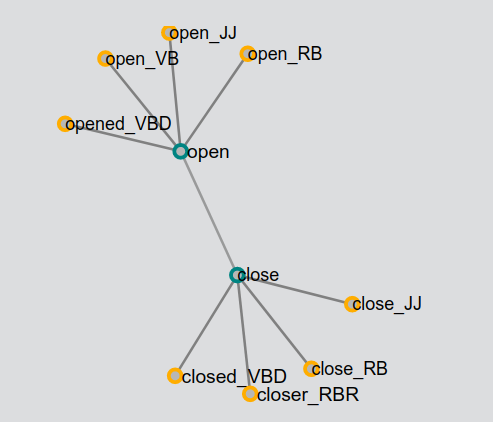
\includegraphics[width=.4\linewidth]{network_1}
  }
  \subfloat[neighbors of \emph{color}]{
    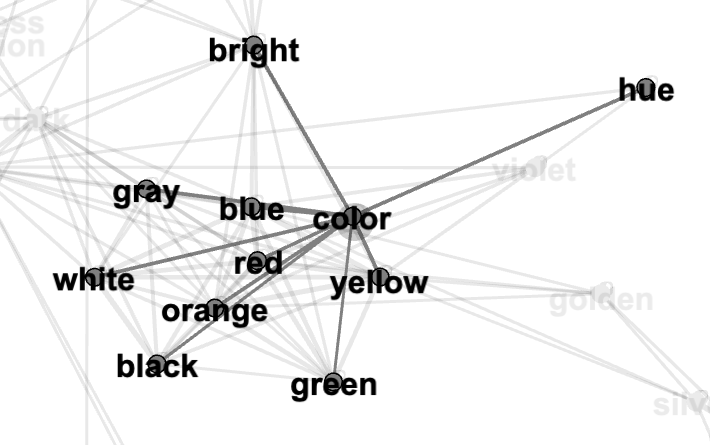
\includegraphics[width=.4\linewidth]{network_2}
  }
  \hspace{0mm}
  \subfloat[neighbors of \emph{noon}]{
    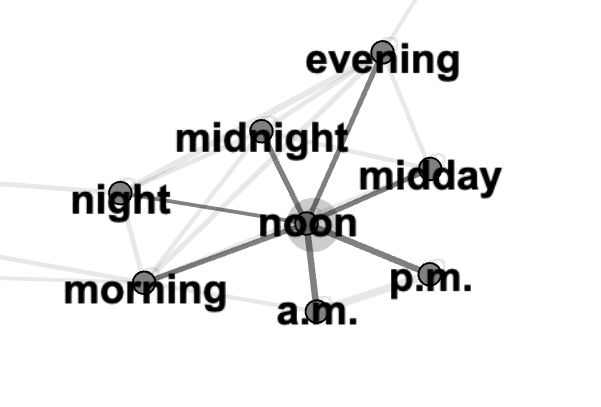
\includegraphics[width=.4\linewidth]{network_3}
  }
  \subfloat[neighbors of \emph{analysis}]{
    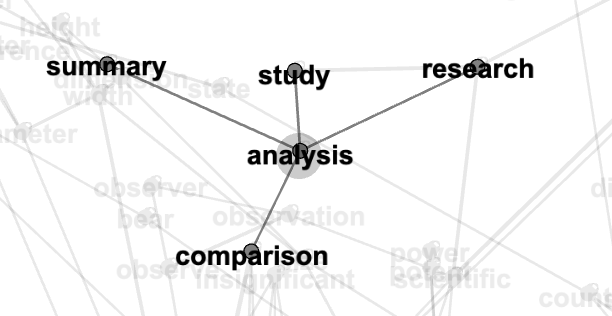
\includegraphics[width=.4\linewidth]{network_4}
  }
  \caption{A figure with two sub-figures}
  \label{fig:network}
\end{figure*}

As we can see in the figure \ref{fig:network} the neighbors of the terms in the
graph are tightly bound with the neighbors that are contextually closer.

By this way we create more structure in the space of vocabulary. Which come
handy in many situations like activity creation, updating mastery of each
vocabulary and analysis. This structure helps in further reducing the search space
by allowing the model to get a better inference about learners level with
relatively very less and effective interactions compared to a method of
tracking each word in the vocabulary individually.


\section{Content organization}

\subsection{Books}
All the processed data such as vocabulary, families, network, sample sentences
are packed into a book instance. This also tracks the meta information such as
Title, Author, Genre, Year and Publisher. This help any future learner to select
the processed book directly. This also could help in comparing the performance
of different learners on the same book.

\subsection{Bookshelf}
All such processed book are organized in multiple bookshelves specific to each
domain similar to the gutenberg project\footnote{\url{http://www.gutenberg.org}}.

\section{Models}
In this work we maintain multiple models to track and update different aspect
of the application.

\subsection{Learner}
The learner instance maintain the personal information of the learner and tracks
the list of instance of books the learner has choose to improve vocabulary and the
progress in them. This also could maintain overall vocabulary knowledge of
the learner and customize the activity type, feedback and book suggestions based
on individual needs.

\subsection{Tutor}
For each book the learner selects, a tutor instance will be created. The main
activities of the tutor are to design a learning session, evaluate the
performance and track the mastery level of the learner w.r.t all the vocabulary
in the book. Then again generate a new session based on the updated mastery
levels in the network.

\textbf{Mastery Score:} The value ranges between 0 and 1. Initially it is
assigned to 0.5 to indicate the uncertainty. Based on the performance of the
learner it is either increased or decreased by a factor. This approach implicitly
capture the un-visited nodes in the network.

\textbf{Update rule:} As we have built a network of families capturing the
contextual similarity. We can incorporate this into our update rule to update
the mastery scores. When we get some outcome for an activity involving a member
from the family ${F_i}$.

\begin{equation}
  M_j = M_j * (1 + (\alpha * sign * S_{ij}))
\end{equation}

Where ${M_i}$ is the mastery of the family ${F_i}$. ${\alpha}$ is a tunable parameter
for the magnitude of an update. ${sign \epsilon \{-1, +1\}}$ is the direction 
of the update. It depends on the correctness of learner response to the corresponding
activity. And ${S_{ij}}$ is the measure of contextual similarity between the two
families ${F_i}$ and ${F_j}$.

\subsection{Session}
An instance of session is created by the tutor. Which decided list of word
families to be practiced. The key functions of this model are to deciding the
interaction type (teaching, testing, feedback), compose an interaction with all
required data and handles the flow and closure of the session.

In order to make the learning more efficient the most critical nodes of the
graph are selected for a session. Here, The criticality of a node is decided
based on the intrinsic(complexity) and extrinsic(degree, quality of connection)
nature of the node.


\section{Activity}
Since our motive is to reduce the effort for content creation. We generate the
activities on the fly. In this work we generate two type of activities. 

\textbf{fit to context:} The learner is prompted to complete 3-4 incomplete
sentences with one among the given list of word suggestions. The options are
chosen to be contextually tight to improve the quality of the activity and
learning outcome.

\textbf{scrambled word:} The learner is prompted to come up with a word from the
set of characters to complete an incomplete sentence. The words with word length
less than 6 characters are allowed to generate this activity. Since the larger
answer words makes it more ambiguous for the learner to solve.

Currently, the activity types are chosen in random for the answer words of length
more than 6 characters. This could also be enhanced to chose based on the learner
interactions.

\begin{figure}
\begin{tcbraster}[raster columns=1, enhanced, blankest]
\tcbincludegraphics{architecture}
\caption{Architecture of system}

\end{tcbraster}
\end{figure}

\subsection{Distractor selection}
The distractors plays an important role in deciding the quality of the activities.
We take advantage of the network of families we built based on the contextual
closeness to overcome this problem. Here we rank the neighbors of the
answer family and chose a best set below a threshold to avoid the synonyms. From
the best set of families we choose the members which matches the POS tag of the
answer word to make all the distractors coherent.



\begin{figure}
\begin{tcbraster}[raster columns=1, enhanced, blankest]
\tcbincludegraphics{1}
\caption{One of activity in which learner has to select one correct answer that satisfies the all given three sentences}

\tcbincludegraphics{8}
\caption{This is the another type of activity in which learner is given a sentence with scrambled characters as options. Learner has to rearrange them to make correct word that fits that sentence.}

\tcbincludegraphics{5}
\caption{This page shows the stats of uploaded book. Number of families, total number of words, most frequent 20 words.}


\tcbincludegraphics{4}
\caption{This is the library page in which preloaded books can be used for activities without processing that book again.}

\end{tcbraster}
\end{figure}



\begin{figure}
\begin{tcbraster}[raster columns=1, enhanced, blankest]
\tcbincludegraphics{7}
\caption{Learner can select the word complexity according to knowledge level. By default it is "Average".}


\tcbincludegraphics{6}
\caption{This is the list of words that will be used for creating activities. Learner can go through these words for getting insight of words.}

\tcbincludegraphics{3}
\caption{If learner gave correct answer this notification bar will be shown on screen with button to proceed for next question. In the meantime learner can also see the progress by progress bar above activity.}

\tcbincludegraphics{2}
\caption{If learner gave wrong answer, this type of notification bar will be shown with another sentence that includes the selected option for actual activity to show how can we use the selected option in future activities.}
\end{tcbraster}
\end{figure}


\section{System Architecture}
Our plan for system was to create interactive and single page application so we used React.js with Redux as frontend for our system. We used CSS for creating animations or user interface. For backend we used Python-Django. We used Rest framework for the interaction between frontend and backend. Controllers in Django handled the request from frontend and then redirected to appropriate API. Django system was also interacting with our proposed vocabulary learning algorithms. We used NoSQL-MongoDB for storing sessions.   



\subsection{System Flow}
The first screen of system is the form in which learner will fill some details like name of author, name of book, publisher, etc. and also upload the book. The next step is to process the book and assign an ID for library reference. Learner can see the stats of book with details like number of families, total number of words, most frequent 20 words. 
The next screen is the list of 20 words that will be used in activities. In the mean time learner can click on various menu items like "Books" for opening library and changing the book or learner can change the complexity level of words by clicking on profile name. The next screen after stats is activity page. There are currently two types of activities which are coming from backend randomly. We are keeping the progress of learner and showing for motivation and also showing learner appropriate error or success message and also giving correct explanation in the case of wrong answer selected. 


\section{Future Work}
The system has limitation on operating on the words that does not have a learned
representation on the vector space. Which could be rectified by learning a
custom word vector specific to the domain. This feature could create new use case
like a tool to learn jargon specifics to a new domain.

Teaching the word in a session.
Control over the complexity (tune-able complexity)
Tracking words at learner level across books (to have a warm start for new book)

On the user interface mobile application can used to attract for learners. The number activity types are limited for now but future work can be implementation of other activity types. Currently this system is one learner limited but after implementation of login screen and maintaining the database of learners with sessions can also be a helpful feature. Use of text to speech can improve learner's pronunciation. 

Integration of forget factor to the learner model as a function of number of days of inactivity.
Extending as a tool to acquire the pre-requisites: Like acquiring commonly used proper nouns specific to a place before going to the place; Getting introduced to nouns and verbs specific to a novel or tv series.


% include your own bib file like this:
\bibliography{vocabby}
\bibliographystyle{vocabby_natbib}
\end{document}
